\input{{configplaindocEN.texconf}}

\usepackage{float}

\author{Lucas Haupt\\ Alexander Koschenko\\ David Mertens\\ Dennis Oberst\\ Lena Marie Wilbertz}
\title{Team Organisation PAM3\\ Mobile Hardware Sampler}
\date{\today}

% Style: Sentence Case (only first word in headings capitalized)

\begin{document}
\maketitle

\section{Specified rules and techniques}

In order to keep a decent project structure and organisation we decided on the following:

\begin{itemize}
	\item Using a platform to keep an overview over the whole project, individual tasks and time everyone spent working on them
	\item Structuring the project into the following parts and preliminary subtasks
	\begin{table}[!h]
	\centering
	\begin{tabular}{l|c|l}
	\textbf{project part} & \textbf{people} & \textbf{subtasks} \\
	\hline
	MIDI and MIDI circuit  & Lena, David & soldering and testing MIDI plug/circuit \\
	Audio & Lucas, Dennis & reading/writing from/to RAM and flash storage, playback \\
	Display & Alex, Dennis & display controls and user interface \\
	\end{tabular}
	\caption{first project structure}\label{tbl:struct}
	\end{table}

	\item First early draft/ideas on how to put things together (fig. \ref{fig:disp} and \ref{fig:draft})
	\begin{figure}[H]
	\centering
	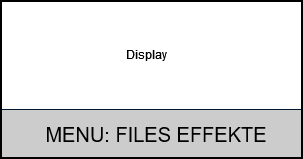
\includegraphics[width=0.25\textwidth]{draft02.png}
	\caption{display draft}\label{fig:disp}
	\end{figure}
	\begin{figure}[H]
	\centering
	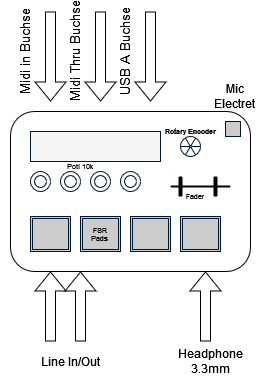
\includegraphics[width=0.25\textwidth]{draft01.png}
	\caption{First draft}\label{fig:draft}
	\end{figure}

\end{itemize}

\section{Things that are still unclear}

\subsection{Documentstyle}
Are there any specific requirements for the documents that are to be uploaded in ILIAS? Do they have to fit a specific formatting, do they all have to be equally formatted and match some style guide?

\subsection{Order of hardware parts}
This will hopefully be discussed in another meeting with Mr. Reiter but there have been some problems in finding the parts at the given stores as well as some considerations on how to split the order in order to keep the costs low.

\section{Problems}
Most problems will come with further progress of the project. For now the biggest challenge we face is to get the signal processing and computing performance of the teensy right. 

Furthermore the challenge will be to design a proper interface (in terms of what the display shows and how to place and assign the buttons) and to make a basic version of the sampler work as described in stage 1 of our project goals.

\section{Possible approaches to solve them}
In order to balance signal processing and computing load of the teensy we will test different approaches of parallel programming with the multithreading library of the teensy.

The people working on the display will examine the possibilities we have depending on the hardware parts and in particular the display size. The other subgroups will work on making the midi interface work and handling data flow and playback on the teensy chip accordingly.

\end{document}
